\section{Discovery: an architectural proposal}
\label{sec:architecture}

\subsection{Related work}

% \begin{itemize}

% 	\item Moreno made a proposition of IaaS architecture \cite{moreno2012iaas}.	
	
% 	\item He identified a list of services that are vital for building IaaS that will be usable in production condition for commercial company.

% 	\item We aim at making a research prototype: we want to keep concepts that are vital for a first prototype:

% 		\begin{description}

% 			\item [Virtual Machine] : Prototype will enable reasearchers to access a big compute power.

% 			\item [Virtual Network] : In addition to infrastructure network, we want to connect virtual machines on an isolated network.

% 			\item [Image disk and persistent storage] : 
% 				\begin{itemize}

% 					\item Virtual machines will be based on images

% 					\item Virtual machines' states are savable.
				
% 				\end{itemize}

% 			\item [Simple authentication] : User will have to authenticate to access prototype. Once they are authenticated they will be able to create virtual machines.

% 		\end{description}

% \end{itemize}


In \cite{moreno2012iaas}, authors have depicted a reference architecture for 
Cloud OS: they aimed at providing an abstraction of underlying technologies that
compose current IaaS managers. The strength of their work resides in the fact
that they considered all the needs of an "industrial class" IaaS manager: every
single function of a cloud is considered and well detailed. That is why we think
that a new architectural proposition should leverage this work.

However, as we aim at making a research prototype, we will volontarily neglect
advanced services in order to focus on those which are vitals, in order to 
propose ana architecure for a simple but working massively distributed IaaS
manager. We also keep in mind that the architecture should be flexible enough to
later include these advanced services in a painless way.

As we target a first prototype that will be able to allow users to manage 
interconnected virtual machines (virtual environment), we only keep services 
that have utility for this purpose. To determine which services are needed, we
have profiled concepts that are involved in the first prototype we target:

\label{cloud_os_concepts}

\begin{description}

	\item [Virtual Machine] : It is the key concept of the system we aim
	to build. In the same way a modern operating systems provides 
	computing resources by provisioning thread, the Cloud OS will 
	produce virtual machines.

	\item [Virtual Network] : Virtual machines of a same virtual 
	environment need to be interconnected. This interconnection will be
	performed by virtual networks.

	\item [Image disk and persistent] : Virtual machines are based on 
	disk images which are specified at creation. It means that a the 
	Cloud OS must propose a storage services for storing reference disk
	images. However this is not enough: a virtual machine can be
	snapshotted, which means that the Cloud OS must provides efficient
	way to persist these states.

	\item [Simple authentication] : As virtual machines provisioning is
	invocked by users, an authentication process is needed to guarantee
	the fairness of resource allocation. This authentication process
	will also have to handle user's role such as customer and Cloud OS's
	administrator.

\end{description}





\subsection{First iteration on the LUC-OS architecture}

% \begin{itemize}

% 	\item For our first iteration, we keep 4 main services:
% 		\begin{description}

% 			\item [Compute manager] : responsible for virtual machines lifecycle.

% 			\item [Network manager] : responsible for virtual networks.

% 			\item [Storage manager] : responsible for images and persistent block storage.

% 			\item [Administrative manager] : responsible for infrastructure management and user permissions.  

% 		\end{description}


% 	\item In figure \ref{fig:mcd} we propose a conceptual data model to explain our proposal.




% 	\item Virtual environment concept is the keystone of the Discovery proposal:
		
% 		\begin{itemize}

% 			\item When a user request the creation of virtual machines for a specified date, an allocation is registered.

% 			\item When the start date is reached, a virtual environment (isolated container for a VLAN and VMs) is created.

% 			\item a virtual environment can be run on several hosts, possibly spread over several geographical sites.

% 		\end{itemize}

% 	\item + description of other entities.

% \end{itemize}

\begin{figure*}
	\centering
	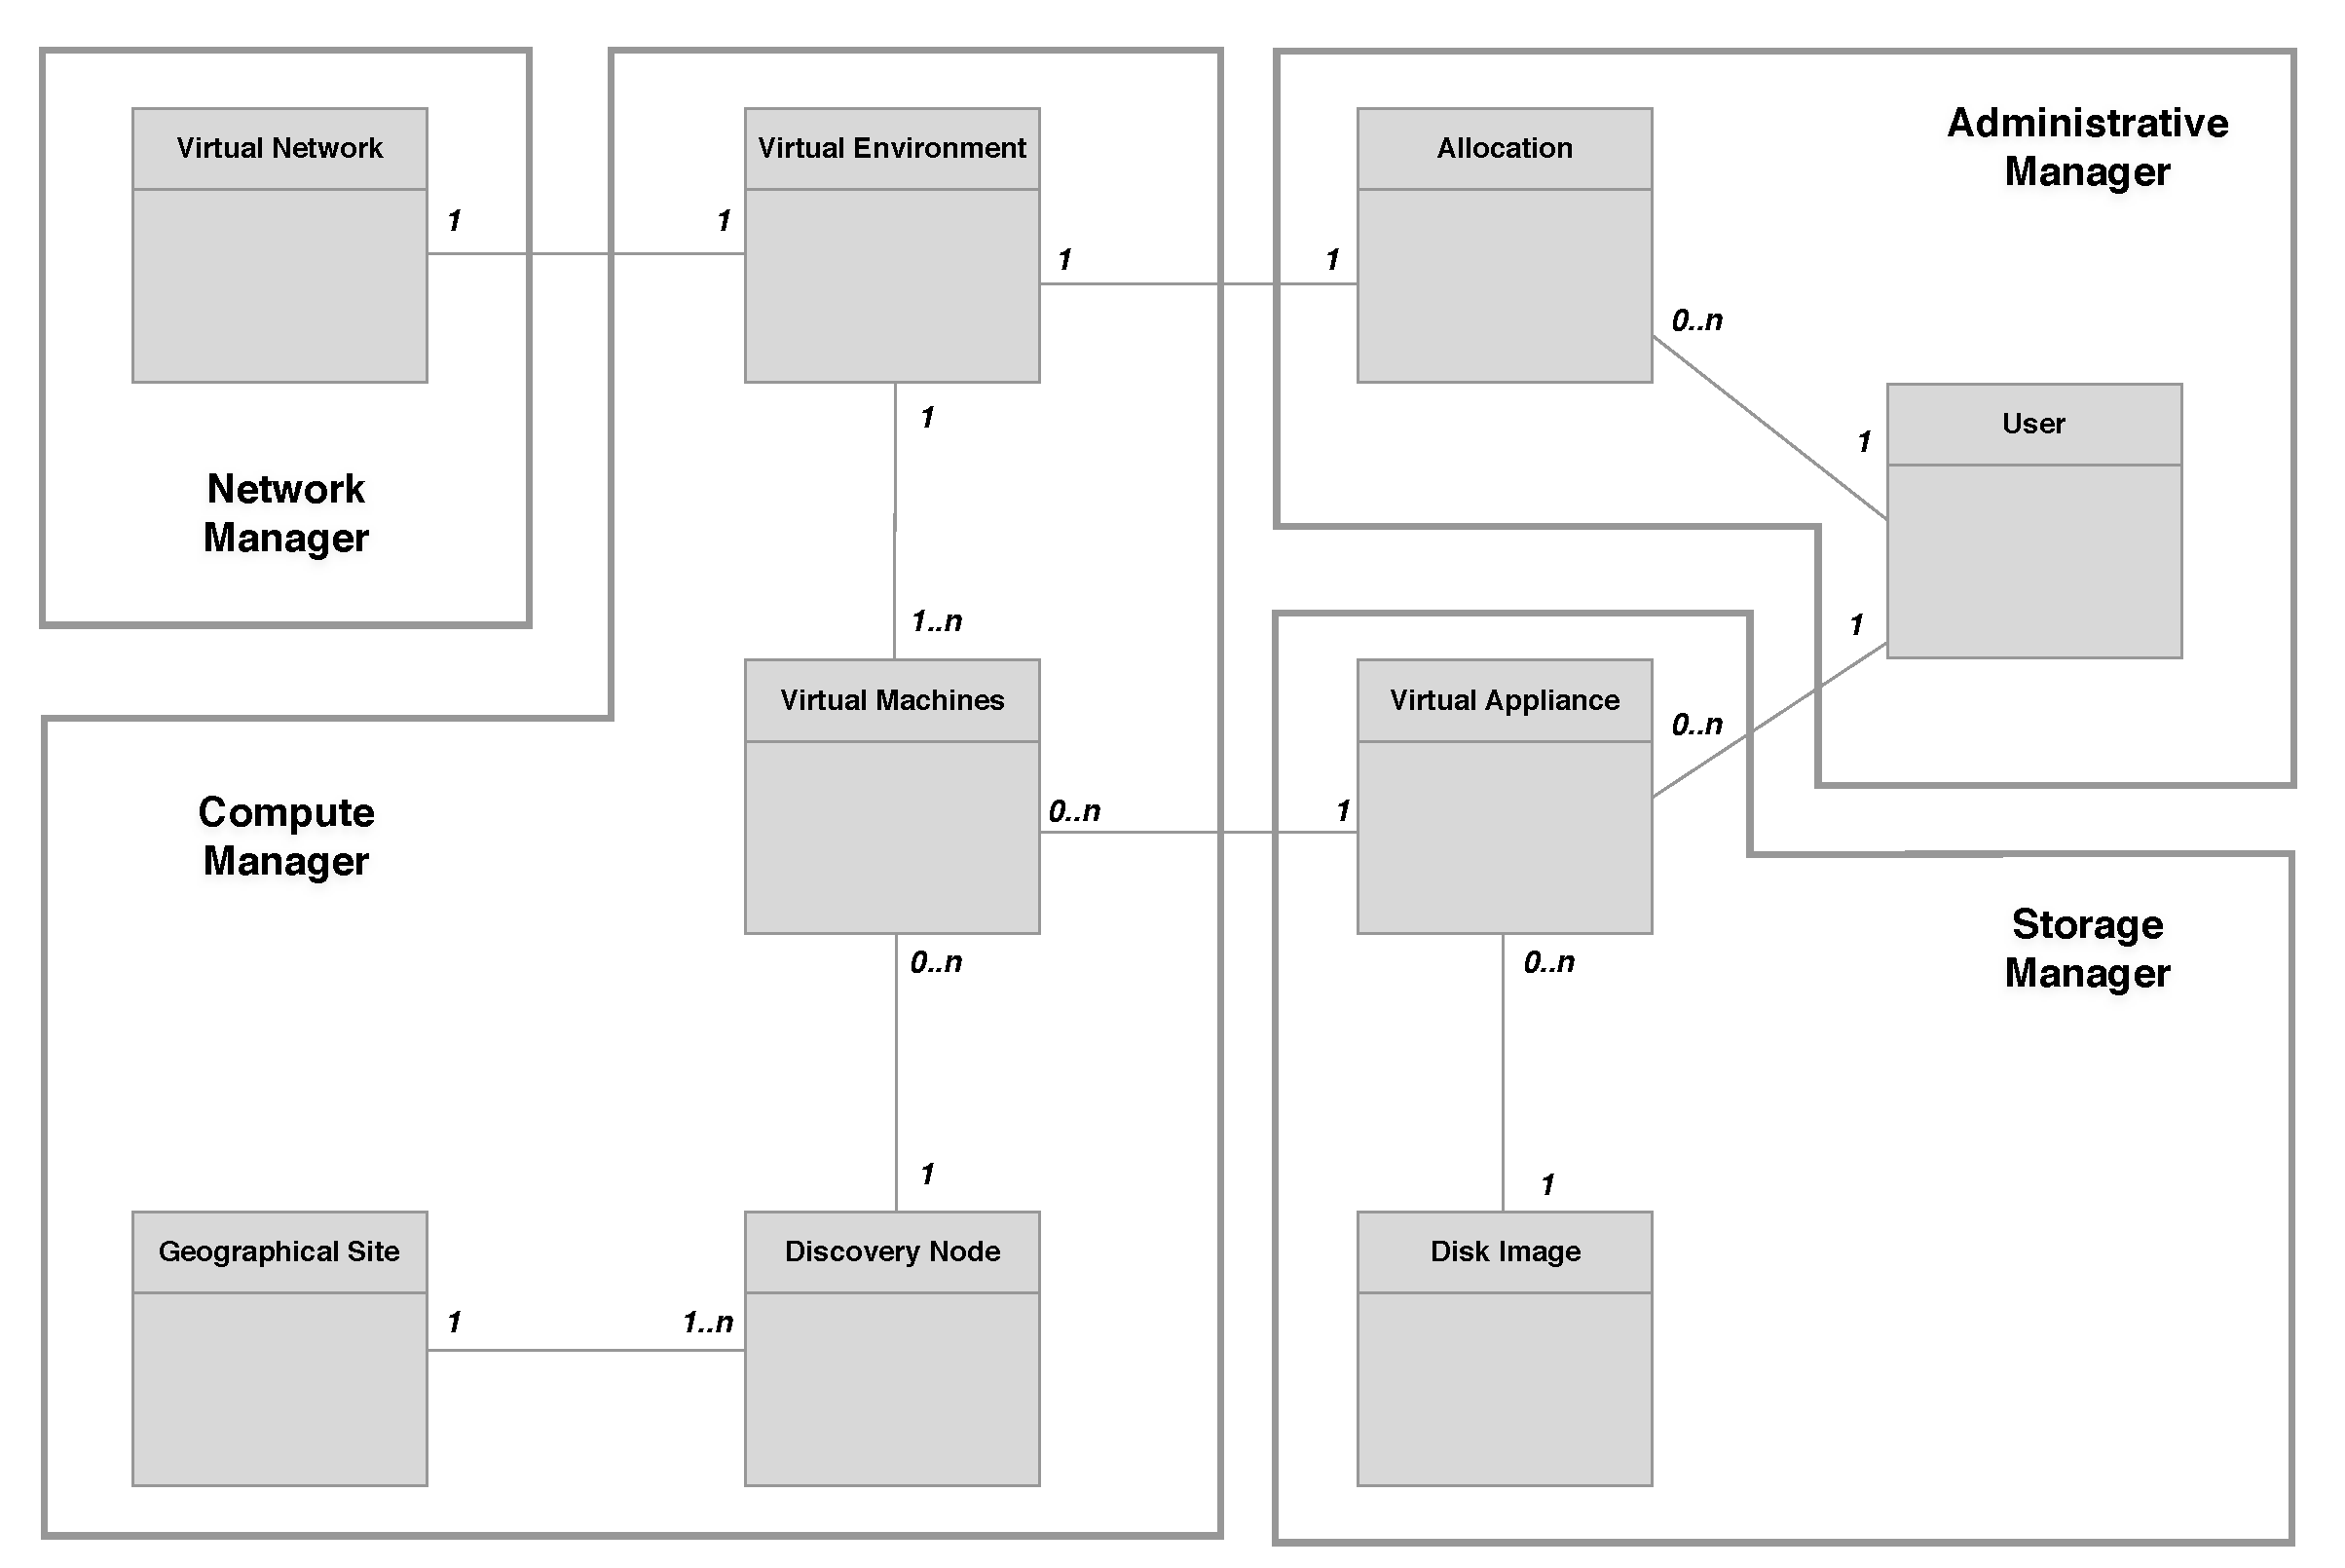
\includegraphics[width=0.91\linewidth]{Figures/mcd_3.pdf}
	\caption{Conceptual schema of the Discovery proposal.}%
	\label{fig:mcd}%
	%\vspace*{-.8cm}
\end{figure*}

Leveraging the concepts that have been depicted in \ref{cloud_os_concepts}, we 
have decided that the first draft of the LUC-OS architecture will focus on 
fundamental services. Each of these services is described in the following 
listing:

\begin{description}

	\item [Compute service] : manage virtual machines' lifecycle.

	\item [Network service] : manage virtual networks.

	\item [Storage service] : manage images and block storage.

	\item [Administrative service] : manage infrastructure and user permissions.  

\end{description}

In figure \ref{fig:mcd} we propose a conceptual schema that enables an easier 
illustration of data concepts, and their relationships, that we plan to use in
the LUC-OS. This is a high-level description which has to purpose to define and 
explain semantics of our proposal. It is noticeable that this schema is 
partitioned in four block corresponding to the previous services.

As we know entities that will be manipulated by the different services of the
Cloud OS, we can give an overview of how entities are involved during virtual
machines provisioning:

\begin{itemize}

	\item A user asks the LUC-OS for some computing resources for a date: 
	the \textbf{administrative service} considers the demand and determine 
	wether it is possible to provide enough resources or not. Once the demand is
	considered as acceptable, an allocation is created and stored in the 
	LUC-OS's data structure (a Distributed Hash Table). To enable accounting 
	operation such as billing, the allocation will be stored long enough.

	\item Once the allocation date has been reached, the \textbf{compute
	service} will ask the dynamic virtual machine scheduler (DVMS) to elect a 
	set of servers that is suitable to spawn the virtual machines, leading to 
	the creation of a new virtual environment which is distributed on the 
	elected servers. \textbf{Network service} then create a new virtual	network
	that is attached to the virtual	environment: during their creation, virtual
	machines will be inter-connected through this virtual network.

	\item The \textbf{storage service} is involved in processes for creating and 
	snapshotting virtual machines. As virtual machine are created from a virtual
	disk image, users will have to specify a virtual appliance which represents
	a disk image base which have been flavoured with some pre-installed 
	software. Once a virtual machine is started, it is possible for users to
	perform snapshot of virtual machines: the state of the virtual machine is
	saved in distributed data structure.

\end{itemize}







